\documentclass[hyperref,titlepage,UTF8]{ctexart}

\usepackage{graphicx}
\usepackage{float}
\usepackage{caption}
\usepackage{amsmath}
\usepackage{multirow}
\usepackage{booktabs}
\usepackage{array}
\usepackage{listings}
\usepackage{color}
\usepackage{pgfplots}
\usepackage{pstricks}
\usepackage{tikz}
\usetikzlibrary{arrows,decorations.pathmorphing,backgrounds,positioning,fit,petri,shapes,snakes,calc}
\usepackage{fontspec}
\setmainfont{Times New Roman}

\definecolor{codegreen}{rgb}{0,0.6,0}
\definecolor{codegray}{rgb}{0.5,0.5,0.5}
\definecolor{codepurple}{rgb}{0.58,0,0.82}
\definecolor{backcolour}{rgb}{0.95,0.95,0.92}

%设计页面尺寸
\usepackage{geometry}
\geometry{a4paper,left=2.5cm,right=2cm,top=2cm,bottom=2cm}
\usepackage{fancyhdr}
\pagestyle{fancy}
\fancyhf{}
\cfoot{\thepage}
\fancyhead[C]{防灾科技学院毕业设计}

%设置目录格式
\usepackage{tocloft}
\setlength\cftbeforepartskip{0.3em}
\setlength\cftbeforesecskip{0.3em}
\setlength\cftbeforesubsecskip{0.3em}
\setlength\cftbeforesubsubsecskip{0.3em}
\renewcommand\cftpartleader{\cftdotfill{\cftpartdotsep}}
\renewcommand\cftpartdotsep{\cftdotsep}
\renewcommand\cftsecleader{\cftdotfill{\cftsecdotsep}}
\renewcommand\cftsecdotsep{\cftdotsep}
\renewcommand\cftpartfont{\bfseries\zihao{4}}
\renewcommand\cftsecfont{\bfseries\zihao{4}}

%设计章节格式
\CTEXsetup[format={\bfseries\zihao{4}}]{paragraph}
\CTEXsetup[format={\bfseries\zihao{4}},indent={0pc},beforeskip={0.3em},afterskip={0.3em}]{part}
\CTEXsetup[format={\bfseries\zihao{4}},indent={0pc},beforeskip={0.3em},afterskip={0.3em}]{section}
\CTEXsetup[format={\bfseries\zihao{-4}},indent={0pc},beforeskip={0.3em},afterskip={0.3em}]{subsection}
\CTEXsetup[format={\bfseries\zihao{-4}},indent={0pc},beforeskip={0.3em},afterskip={0.3em}]{subsubsection}

%书签和文档信息设置
\hypersetup{linkcolor=black,anchorcolor=black,filecolor=black,urlcolor=black,citecolor=black,bookmarksopen=true,pdftitle={基于GUI的误差理论与数据处理},pdfauthor={艾江南},pdfsubject={防灾科技学院毕业论文}}

%代码高亮设计
\lstset{columns=flexible,
	language=Matlab,
%	escapechar=',
	backgroundcolor=\color{backcolour},
	keywordstyle=\color{magenta},
%	numberstyle=\small\color{codegray},
	stringstyle=\color{codepurple},
	commentstyle=\color{codegreen},
	basicstyle=\small,
	breakatwhitespace=false,
	breaklines=true,
	captionpos=b,
	keepspaces=true,
%	numbers=left,
%	numbersep=8pt,
	showspaces=false,
	showstringspaces=false,
	showtabs=false,
	tabsize=4}

%定制命令
\newcommand\scite[1]{\textsuperscript{\cite{#1}}}
\newcommand{\tabincell}[2]{\begin{tabular}{@{}#1@{}}#2\end{tabular}}

%\includeonly{前言}
%\includeonly{引言}
%\includeonly{内容1}
%\includeonly{内容2}
%\includeonly{结论}
%\includeonly{致谢}
%\includeonly{参考文献}
%\includeonly{附录}

\begin{document}
\zihao{-4}
\pdfbookmark[0]{封面}{titlepage}
\begin{titlepage}
	\rightline{
\includegraphics[scale=0.6]{logo}}
	\begin{center}
		\vspace*{4cm}
		\textbf{\heiti \zihao{1} 防\enspace 灾\enspace 科\enspace 技\enspace 学\enspace 院}
		
		\vspace*{1cm}
		\textbf{\kaishu \zihao{-0} 毕\enspace 业\enspace 设\enspace 计}
		
		\vspace*{6cm}
	\begin{tabular}{cp{4cm}cp{4cm}}
		\textbf{\zihao{4} 题\qquad 目}&\multicolumn{3}{c}{\zihao{4} 基于GUI的误差理论与数据处理}\\\cline{2-4}
		&&&\\
		\textbf{\zihao{4} 学生姓名}&\multicolumn{1}{c}{\zihao{4} 艾江南}&\textbf{\zihao{4} 学\qquad 号}&\multicolumn{1}{c}{\zihao{4} 135032105}\\\cline{2-2}\cline{4-4}
		&&&\\
		\textbf{\zihao{4} 班\qquad 级}&\multicolumn{1}{c}{\zihao{4} 1350321}&\textbf{\zihao{4} 专\qquad 业}&\multicolumn{1}{c}{\zihao{4} 测控技术与仪器}\\\cline{2-2}\cline{4-4}
		&&&\\
		\textbf{\zihao{4} 系\qquad 别}&\multicolumn{3}{c}{\zihao{4} 防灾仪器系}\\\cline{2-4}
		&&&\\
		\textbf{\zihao{4} 开题时间}&\multicolumn{1}{c}{\zihao{4} 2016年12月26日}&\textbf{\zihao{4} 答辩时间}&\multicolumn{1}{c}{\zihao{4} 2017年x月x日}\\\cline{2-2}\cline{4-4}
		&&&\\
		\textbf{\zihao{4} 指导教师}&\multicolumn{1}{c}{\zihao{4} 姚振静}&\textbf{\zihao{4} 职\qquad 称}&\multicolumn{1}{c}{\zihao{4} 副教授}\\\cline{2-2}\cline{4-4}
	\end{tabular}
	\end{center}
\end{titlepage}
\newpage
\thispagestyle{empty}
\pdfbookmark[0]{摘要}{center}
\begin{center}
	\textbf{\heiti \zihao{3} 基于GUI的误差理论与数据处理}
	
	\vspace{1em}
	作\qquad 者\quad 艾江南
	
	指导老师\quad 姚振静
\end{center}
\vspace{2em}
\paragraph{摘要}{\kaishu \zihao{5} 这是摘要。。。不超过300汉字,五号楷体}
\vspace{2em}
\paragraph{关键词:}\textbf{\zihao{4} 关键词1;关键词2;关键词3}
\newpage
\thispagestyle{empty}
\pdfbookmark[0]{Abstract}{0}
\begin{center}
	\textbf{\heiti \zihao{3} Title:XXXXXXXXXXXXXXXXXXXXXX}
	
	\vspace{1em}
	Author\quad Ai Jiangnan
	
	Tutor\quad Yao zhenjing
\end{center}
\vspace{2em}
\paragraph{Abstract}{\zihao{5} XXXXXXXXXXXXXXXXXXXXXXXXX.}
\vspace{2em}
\paragraph{Keywords:}\textbf{\zihao{4} Keywords1;Keywords2;Keywords3}
\newpage
\pdfbookmark[0]{目录}{1}
\begin{center}
	\tableofcontents
\end{center}
\thispagestyle{empty}
\setcounter{page}{1}
\part*{引言}
\addcontentsline{toc}{part}{引言}
这是$ x^2+y^2=z^2 $引言。\[ \sum_{i=1}^{\infty}x^i \]

\section{误差理论与数据处理\scite{1}}
\subsection{误差的基本性质与处理}
\subsubsection{随机误差}
当我们对同一个测量值进行多次的等精度重复测量时,可以得到一系列的不同的测量值,这些测量值多多少少都会存在误差,它们的出现是没有确定的规律的,但对于它们总体而言,却有统计的规律性。

当测量列中不包括系统误差和粗大误差时,随机误差的分布可以是正态分布,也可以是其他分布,比如,均匀分布、三角形分布、$ \chi^2 $分布等,而大多数随机误差都服从正态分布。

假设被测量的真值为$ L_0 $,而测得值为$ l_i(i=1,2,...,n) $,则测量数据的随机误差$ \delta_i $为\[ \delta_i=l_i-L_0 \]

正态分布的分布密度$ f(\delta) $与分布函数$ F(\delta) $为\[ f(\delta)=\frac{1}{\sigma\sqrt{2\pi}}e^{-\delta^2/(2\sigma^2)} \]\[ F(\delta)=\frac{1}{\sigma\sqrt{2\pi}}\int_{-\infty}^{\delta}e^{-\delta^2/(2\sigma^2)}d\delta \]
式中:$ \sigma $为总体标准差,$ e $为自然对数底。
\begin{enumerate}
	\item \textbf{算术平均值}
	
	\qquad 在一系列的测量值中,被测量的$ n $个测得值的代数和除以$ n $而得的值称为算术平均值\footnote{《误差理论与数据处理》第22页算术平均值的定义,详情见参考文献[1]}。设$ l_1,l_2,...,l_n $为$ n $次测量所得的值,则算术平均值$ \bar{x} $为\[ \bar{x}=\frac{l_1+l_2+...+l_n}{n}=\frac{1}{n}\sum_{i=1}^{n}l_i \]
	当测量次数无限大时,算术平均值被认为是最接近于真值的。
	\item \textbf{标准差}
	
	\textbf{单次测量的标准差 } 同一个被测量,在相同条件下,测量列$ l_1,l_2,...,l_n $中单次测量的标准差是表征同一被测量$ n $次测量结果分散性的参数,并按下式计算。
	\[ \sigma=\sqrt{\frac{\sum\limits_{i=1}^{n}(l_i-L_0)^2}{n}}=\sqrt{\frac{\sum\limits_{i=1}^{n}\delta_i^2}{n}} \]
	式中:$ n $为测量次数(应充分大);$ \delta_i $为第$ i $个测量值所对应的随机误差,即测量值与被测量值的真值之差。
	
	\qquad 对于标准差恒等的测量,我们把它定义为等精度测量,对于相同的测量条件下所做的重复测量均为等精度测量。反之,则属于不等精度测量。
	
	\qquad 对同一被测量,在相同测量条件下,进行有限次测量得测量列$ l_1,l_2,...,l_n $,则单次测量标准差的估计值为\[ s=\sqrt{\frac{\sum\limits_{i=1}^{n}v_i^2}{n-1}} \]
	这也被叫做贝塞尔公式。
	
	\textbf{算术平均值的标准差 } 算术平均值的标准差$ \bar{s} $则是表征同一被测量的各个独立测量列算术平均值分散的参数。\[ \bar{s}=\frac{s}{\sqrt{n}} \]
	\item \textbf{测量的极限误差}
	
	\textbf{单次测量的极限误差 } 根据概率论知识,已知正态分布曲线可得:\[ p=\int_{-\infty}^{+\infty}f(\delta)d\delta=\int_{-\infty}^{+\infty}\frac{1}{\sigma\sqrt{2\pi}}e^{-\frac{\delta^2}{2\sigma^2}}d\delta=1 \]
	由此,误差落在区间$ [-\delta,+\delta] $之间的概率为:\[ p=\int_{-\delta}^{+\delta}f(\delta)d\delta=\int_{-\delta}^{+\delta}\frac{1}{\sigma\sqrt{2\pi}}e^{-\frac{\delta^2}{2\sigma^2}}d\delta \]
	将上式进行变量转换,设\[ t=\frac{\delta}{\sigma},dt=\frac{d\delta}{\sigma} \]
	经变换,上式成为\[ p=\frac{1}{\sqrt{2\pi}}\int_{-t}^{+t}e^{-\frac{t^2}{2}}dt=\frac{2}{\sqrt{2\pi}}\int_{0}^{+t}e^{-\frac{t^2}{2}}dt=2\Phi(t) \]
	\[ \Phi(t)=\frac{1}{\sqrt{2\pi}}\int_{0}^{+t}e^{-\frac{t^2}{2}}dt \]
	若某随机误差在$ \pm t\sigma $范围内出现的概率为$ 2\Phi(t) $,则超出的概率为\[ \alpha=1-2\Phi(t) \]
	不同的$ t $时超出$ |\delta| $的概率是不同的,取不同的$ t $值时,极限误差可用下式表示:\[ \delta_{lim}x=\pm t\delta \]
	\textbf{算术平均值的极限误差} \[ \delta_{lim}\bar{x}=\pm t_a\sigma_{\bar{x}} \]
	式中:$ t_a $为置信系数;$ \alpha $为超出极限误差的概率;$ \sigma_{\bar{x}} $为$ n $次测量的算术平均值标准差。
	\item \textbf{权}
	
	\qquad 在等精度测量中,各个测得的值我们认为是同样可靠的,用所有值的算术平均值作为最后的测量结果。但是在不等精度测量中,各个测量值的可靠程度是不一样的,所以我们用权来说明测量的可靠程度。我们根据算术平均值标准差以及测量的次数来确定权,假设同一测量量有$ m $组不等精度的测量结果,可表示为\[ p_1:p_2:...:p_m=\frac{1}{\sigma_{\bar{x_1}}^2}:\frac{1}{\sigma_{\bar{x_2}}^2}:...:\frac{1}{\sigma_{\bar{x_m}}^2} \]
	\item \textbf{加权算术平均值}
	
	\qquad 在对m组测量量进行不等精度的测量时,得到的结果是$ \bar{x_1},\bar{x_2},...,\bar{x_m} $,设相应的测量次数为$ n_1,n_2,...,n_m $,可以得出全部测量的算术平均值为\[ \bar{x}=\frac{\sum\limits_{i=1}^{m}p_i\bar{x}_i}{\sum\limits_{i=1}^{m}p_i} \]
	\item \textbf{加权算术平均值的标准差}\[ \bar{s}=\sqrt{\frac{\sum\limits_{i=1}^{m}p_iv_{\bar{x_i}}^2}{(m-1)\sum\limits_{i=1}^{m}p_i}} \]
\end{enumerate}
\subsubsection{系统误差}
\begin{enumerate}
	\item \textbf{系统误差的产生原因}
	
	\qquad 系统误差是由固定不变的或者是按照确定的规律变化的因素所造成的。它是由多方面因素引起的:测量装置方面,环境方面的因素,测量方法的因素,测量人员方面的因素\footnote{《误差理论与数据处理》第41页,详情见参考文献[1]}。
	\item \textbf{系统误差的发现}
	
	\qquad 发现系统误差的方法有很多种,在组内有,实验对比法、残余误差观察法、残余误差校核法、不同公式计算标准差法;在组间有,计算数据比较法、秩和校验法、$ t $检验法。
	\item \textbf{系统误差的减小与排除}
	
	\qquad 我们要消除系统误差有两种方法,第一种是从产生误差根源上消除,第二种是用修正方法消除系统误差。
	
	\qquad 常用的不变系统误差消除法有:代替法、抵消法、交换法。线性系统误差消除法有:对称法。周期性系统误差消除法有:半周期法。
\end{enumerate}
\subsubsection{粗大误差}
在一系列重复的测量数据中,如果有个别的数据(最大值或最小值)严重地偏离了它所属样本的其他数据,则可以怀疑该组数据中含有粗大误差。
\begin{enumerate}
	\item \textbf{粗大误差产生的原因}
	
	\qquad 产生粗大误差的原因是多方面的,不过大致可以归纳为测量人员的主观原因和客观外界条件的原因。
	\item \textbf{粗大误差的特点}
	
	\qquad 粗大误差的特点可以总结为以下三点,第一,在引起粗大误差的各种因素中,很难事先预测到,所以它具有突发性。第二,产生的粗大误差一般都远大于正常测量值之间的距离,所以它一般为较大的数值。第三,含有粗大误差的异常数据个数一般都很少,所以它有数量少的特点。
	\item \textbf{判别粗大误差的准则}
	
	\qquad 遇到粗大误差时,我们要慎重对待,并要根据判别准则予以确定。通常用来判别粗大误差的准则有:$ 3\sigma $准则(莱以特准则)、罗曼诺夫斯基准则($ t $检验准则)、格拉布斯准则、狄克逊准则、奈尔准则、精细准则、肖维涅准则。
	
	\qquad 我们主要介绍狄克逊准则,因为它不需要事先求出标准差$ \sigma $,而且我们后面用到该方法检验粗大误差。狄克逊研究了$ x_1,x_2,...,x_n $的顺序统计量$ x_{(i)} $的分布,当$ x_{(i)} $服从正态分布时,得到$ x_{(i)} $的统计量
	\[ \begin{cases}
		r_{10}=\frac{x_{(n)}-x_{(n-1)}}{x_{(n)}-x_{(1)}}\\
		r_{11}=\frac{x_{(n)}-x_{(n-1)}}{x_{(n)}-x_{(2)}}\\
		r_{21}=\frac{x_{(n)}-x_{(n-2)}}{x_{(n)}-x_{(2)}}\\
		r_{22}=\frac{x_{(n)}-x_{(n-2)}}{x_{(n)}-x_{(3)}}
	\end{cases} \]
	的分布,选定显著度$ \alpha $,得到统计量的临界值$ r_0(n,\alpha) $,当测量值的统计值$ r_{ij} $大于临界值,则认为$ x_n $含有粗大误差。
	
	\qquad 统计量的临界值$ r_0(n,\alpha) $的查询见附录A 狄克逊检验统计量和临界值。
\end{enumerate}

\subsubsection{等精度测量数据的误差分析}
前面我们讨论了三类测量误差,它们的特点各异,因而处理的方法也有较大差别。等精度测量处理过程如图1所示,我们举一个等精度测量处理过程的例子。
\paragraph{例 } 对某一轴径进行等精度测量9次,得到表1的数据(单位略),求测量结果。

\begin{figure}[H]
	\centering
	\begin{tabular}{|p{3cm}<{\centering}|p{3cm}<{\centering}|p{3cm}<{\centering}|p{3cm}<{\centering}|}
	\hline 
		序号	&  $ l $&  $ v_i $&  $ v_i^2 $\\	\hline 
		1&  24.774&  -0.001&  0.000001\\ \hline 
		2&  24.778&  +0.003&  0.000009\\ \hline 
		3&  24.771&  -0.004&  0.000016\\ \hline
		4&  24.780&  +0.005&  0.000025\\ \hline
		5&  24.772&  -0.003&  0.000009\\ \hline
		6&  24.777&  +0.002&  0.000004\\ \hline
		7&  24.773&  -0.002&  0.000004\\ \hline
		8&  24.775&		  0&  		 0\\ \hline
		9&  24.774&  -0.001&  0.000001\\ \hline
		\multicolumn{4}{|c|}{$ \sum\limits_{i=1}^{9}x_i=222.974,\quad\bar{x}=24.775,\quad\sum\limits_{i=1}^{9}v_i=-0.001,\quad\sum\limits_{i=1}^{9}v_i^2 =0.000069$}\\ \hline
	\end{tabular}
	\captionsetup{type=table}
	\caption{某9次等精度测量数据}
\end{figure}
\begin{figure}[H]
	\centering
	\begin{tikzpicture}[
	>=latex,
	node distance=5mm,
	hv path/.style={to path={-| (\tikztotarget)}},
	vh path/.style={to path={|- (\tikztotarget)}},
	startend/.style={draw,rectangle,rounded corners=2mm,minimum size = 6mm,	thick},
	ioput/.style={draw,trapezium,trapezium left angle=60, trapezium right angle=120,inner sep = 5pt},
	chuli/.style={draw,rectangle,minimum size=6mm,thick},
	panduan/.style={draw,diamond,minimum size=6mm,shape aspect=3,inner sep = 0.1pt,thick}
	]
	\node	(a)		[startend]				{开始};
	\node	(b)		[ioput,below=of a]		{导入测量数据$ l_i(i=1,2,...,n) $};
	\node	(c)		[panduan,below=of b]	{是否有粗大误差?};
	\node	(d)		[chuli,right=of c]		{剔除含有粗大误差数据};
	\node	(e)		[panduan,below=of c]	{是否有系统误差?};
	\node	(f)		[chuli,below=of e]		{计算算术平均值$ \bar{x} $};
	\node	(g)		[chuli,below=of f]		{修正算术平均值$ \bar{x}=\bar{x}+\Delta $};
	\node	(h)		[chuli,below=of g]		{计算单次测量的标准差$ s $};
	\node	(i)		[chuli,below=of h]		{计算算术平均值标准差$ s(\bar{x}) $};
	\node	(j)		[chuli,below=of i]		{根据显著性水平及分布查表得$ t_\alpha $};
	\node	(k)		[chuli,below=of j]		{计算算术平均值极限误差$ \delta_{lim}\bar{x}=\pm t_\alpha s(\bar{x}) $};
	\node	(l)		[chuli,below=of k]		{给出测量结果$ L=\bar{x}+\delta_{lim}\bar{x} $};
	\node	(m)		[startend,below=of l]	{结束};
	
	\draw[->](a)--(b);
	\draw[->](b)--(c);
	\draw[->](c)--(d);
	\path (d.north) edge [->,vh path]($(b.south)!.5!(c.north)$);
	\draw[->](c)--(e);
	\draw[->](e)--(f);
	\draw[->](f)--(g);
	\draw[->](g)--(h);
	\draw[->](h)--(i);
	\draw[->](i)--(j);
	\draw[->](j)--(k);
	\draw[->](k)--(l);
	\draw[->](l)--(m);
	
	\node at (0.25,-3.6){否};
	\node at (2.15,-2.5){是};
	\end{tikzpicture}
	\caption{等精度测量数据处理流程图}
\end{figure}
\begin{enumerate}
	\item \textbf{粗大误差判别(用狄克逊准则差别)}
	
	\qquad 将数据进行从小到大排序,可以得到最小值$ x_{(1)} $和最大值$ x_{(9)} $。\[ x_{(1)}=24.771,x{(9)}=24.780 \]
	首先判断最大值$ x_{(9)} $,因$ n=9 $,帮计算得统计量$ r_{11} $为\[ r_{11}=\frac{x_{(9)}-x_{(8)}}{x_{(9)}-x_{(2)}}=\frac{24.780-24.778}{24.780-24.772}=\frac{0.002}{0.008}=0.400 \]
	查狄克逊准则临界表\footnote{见附录A}可知\[ r_0(9,0.05)=0.512 \]\[ r_{11}=0.4<r_0(9,0.05)=0.512 \]
	可以判断最大值$ x_{(9)} $不含有粗大误差,再对最小值$ x_{(1)} $计算相应统计量$ r'_{11} $
	\[ r'_{11}=\frac{x_{(1)}-x_{(2)}}{x_{(1)}-x_{(8)}}=\frac{24.771-24.772}{24.771-24.778}=\frac{-0.001}{-0.005}=0.167 \]
	\[ r'_{11}=0.167<r_0(9,0.05)=0.512 \]
	可以判断最小值$ x_{(1)} $不含有粗大误差,故可以判断该测量数据不含有粗大误差。
	\item \textbf{系统误差差别(用残余误差观察法)}
	
	\qquad 如图2所示,发现残余误差大体相同,无明显变化规律,可以认为不存在系统误差。
	\begin{figure}[H]
		\centering
		\begin{tikzpicture}
			\begin{axis}[ymajorgrids,minor tick num=1,width=15cm,height=7cm]
				\addplot[only marks] coordinates {
					(1,-0.001)
					(2,0.003)
					(3,-0.004)
					(4,0.005)
					(5,-0.003)
					(6,0.002)
					(7,-0.002)
					(8,0)
					(9,-0.001)
				};
			\end{axis}
		\end{tikzpicture}
		\caption{残余误差分布}
	\end{figure}

	\item \textbf{随机误差处理}
		\begin{enumerate}
			\item 求算术平均值:\[ \bar{x}=\frac{\sum\limits_{i=1}^{n}l_i}{n}=\frac{222.974}{9}mm=24.7749mm\approx24.775mm \]
			\item 求残余误差(见列表):\[ v_i=l_i-\bar{x} \]
			\item 校核算术平均值和残余误差。\[ \left| \sum\limits_{i=1}^{9}v_i \right|=0.001mm<\left(\frac{n}{2}-0.5\right)A=4\times0.001mm=0.004mm  \]
			以上计算正确,否则,应重新进行计算和校核:
			\item 求单次测量的标准差(贝塞尔公式)\[ s=\sqrt{\frac{\sum\limits_{i=1}^{n}v_i^2}{n-1}}=\sqrt{\frac{0.000069}{8}mm^2}=0.0029mm \]
			\item 求算术平均值的标准差:\[ \bar{s}=\frac{s}{\sqrt{n}}\approx0.001mm \]
			\item 求算术平均值的极限误差。
			
			\qquad 因为测量的次数较少,算术平均值的极限误差按$ t $分布计算,已知$ v=n-1=8 $,取$ \alpha=0.05 $查得$ t $分布临界值表得$ t_\alpha=2.31 $,则算术平均值的极限误差$ \delta_{lim}\bar{x} $为\[ \delta_{lim}\bar{x}=\pm t_\alpha\sigma_{\bar{x}}=\pm2.31\times0.001mm=\pm0.0023mm \]
		\end{enumerate}
	\item \textbf{测量结果}\[ L=\bar{x}\pm\delta_{lim}\bar{x}=(24.755\pm0.0023)mm \]
\end{enumerate}
\subsubsection{不等精度测量数据的误差分析}
\begin{figure}[H]
	\centering
	\begin{tikzpicture}[
	>=latex,
	node distance=5mm,
	hv path/.style={to path={-| (\tikztotarget)}},
	vh path/.style={to path={|- (\tikztotarget)}},
	startend/.style={draw,rectangle,rounded corners=2mm,minimum size = 6mm,	thick},
	ioput/.style={draw,trapezium,trapezium left angle=60, trapezium right angle=120,inner sep = 5pt},
	chuli/.style={draw,rectangle,minimum size=6mm,thick},
	panduan/.style={draw,diamond,minimum size=6mm,shape aspect=3,inner sep = 0.1pt,thick}
	]
	\node	(a)		[startend]				{开始};
	\node	(b)		[ioput,below=of a]		{导入测量数据$ L_i(i=1,2,...,m) $};
	\node at (-4,-2.4)	(cl)	[chuli]		{计算算术平均值$ \bar{x_1} $};
	\node at (4,-2.4)	(cr)	[chuli]		{计算算术平均值$ \bar{x_m} $};
	\node	(dl)	[panduan,below=of cl]	{是否有粗大误差?};
	\node	(dr)	[panduan,below=of cr]	{是否有粗大误差?};
	\node	(el)	[chuli,right=of dl,align=center]		{剔除含有粗\\大误差数据};
	\node	(er)	[chuli,right=of dr,align=center]		{剔除含有粗\\大误差数据};
	\node	(fl)	[panduan,below=of dl]	{是否有系统误差?};
	\node	(fr)	[panduan,below=of dr]	{是否有系统误差?};
	\node	(gl)	[chuli,below=of fl]		{修正算术平均值$ \bar{x_1}=\bar{x_1}+\Delta_1 $};
	\node	(gr)	[chuli,below=of fr]		{修正算术平均值$ \bar{x_m}=\bar{x_m}+\Delta_m $};
	\node	(hl)	[chuli,below=of gl]		{计算单次测量的标准差$ s_1 $};
	\node	(hr)	[chuli,below=of gr]		{计算单次测量的标准差$ s_m $};
	\node	(il)	[chuli,below=of hl]		{计算加权算术平均值标准差$ s(\bar{x_1}) $};
	\node	(ir)	[chuli,below=of hr]		{计算加权算术平均值标准差$ s(\bar{x_m}) $};
	\node	(jl)	[chuli,below=of il]		{计算相应的权$ p_1=1/(s(\bar{x_1}))^2 $};
	\node	(jr)	[chuli,below=of ir]		{计算相应的权$ p_m=1/(s(\bar{x_m}))^2 $};
	\node at (0,-12)	(k)		[chuli]		{计算加权算术平均值$ \bar{x}=\frac{\sum\limits_{i=1}^{m}p_i\bar{x_i}}{\sum\limits_{i=1}^{m}p_i} $};
	\node	(l)		[chuli,below=of k]		{计算加权算术平均值标准差$ \bar{s}=\bar{s_i}\sqrt{\frac{p_i}{\sum\limits_{i=1}^{m}p_i}} $};
	\node	(m)		[chuli,below=of l]		{计算加权算术平均值极限误差$ \delta_{lim}\bar{x}=\pm t_\alpha s(\bar{x}) $};
	\node	(n)		[chuli,below=of m]		{给出测量结果$ L=\bar{x}+\delta_{lim}\bar{x} $};
	\node	(o)		[startend,below=of n]	{结束};

	\draw[->](a)--(b);
	\path (b) edge [->,hv path](cl);
	\path (b) edge [->,hv path](cr);
	\draw[->](cl)--(dl);\draw[->](cr)--(dr);
	\draw[->](dl)--(el);\draw[->](dr)--(er);
	\path (el) edge [->,vh path](cl);
	\path (er) edge [->,vh path](cr);
	\draw[->](dl)--(fl);\draw[->](dr)--(fr);
	\draw[->](fl)--(gl);\draw[->](fr)--(gr);
	\draw[->](gl)--(hl);\draw[->](gr)--(hr);
	\draw[->](hl)--(il);\draw[->](hr)--(ir);
	\draw[->](il)--(jl);\draw[->](ir)--(jr);
	\path (jl) edge [->,vh path](k);
	\path (jr) edge [->,vh path](k);
	\draw[->](k)--(l);
	\draw[->](l)--(m);
	\draw[->](m)--(n);
	\draw[->](n)--(o);

	\node at (-1.9,-3.6){是};
	\node at (6.1,-3.6){是};
	\node at (-3.8,-4.8){否};
	\node at (4.2,-4.8){否};
	\node at (-3.8,-6.6){是};
	\node at (4.2,-6.6){是};
	\end{tikzpicture}
	\caption{不等精度测量数据处理流程图}
\end{figure}
\paragraph{例}对某一角度进行6组不等精度的测量,假设不含有随机误差和系统误差,各组测量的数据如下:

测6次得$ \alpha_1=75^\circ18'16'' $,测30次得$ \alpha_2=75^\circ18'10'' $,测24次得$ \alpha_3=75^\circ18'08'' $,测12次得$ \alpha_4=75^\circ18'16'' $,测12次得$ \alpha_5=75^\circ18'13'' $,测36次得$ \alpha_6=75^\circ18'09'' $,求得最后的测量结果。
\begin{enumerate}
	\item 根据测量的数据求出各组的权,有\[ p_1:p_2:p_3:p_4:p_5:p_6=1:5:4:2:2:6 \]取\[ p_1=1,p_2=5,p_3=4,p_4=2,p_5=2,p_6=6 \]
	\item 求出加权算术平均值$ \bar{\alpha} $:\[ \bar{\alpha}=\sum_{i=1}^{6}p_i\alpha_i=75^\circ18'10'' \]
	\item 求残余误差,由公式$ v_i=\alpha_i-\bar{\alpha} $得\[ v_1=-4'',v_2=0,v_3=-2'',v_4=6'',v_5=3'',v_6=-1'' \]
	\item 校核算术平均值及残余误差。用加权残余误差代数和等于0来校核。因:\[ \sum_{i=1}^{6}p_iv_i=0 \]所以计算正确。
	\item 求加权算术平均值的标准差:\[ \bar{s}=\sqrt{\frac{\sum\limits_{i=1}^{6}p_iv_i^2}{(m-1)\sum\limits_{i=1}^{6}p_i}}=1.1'' \]
	\item 求加权算术平均值的极限误差,我们可以根据测量数据得出,该数据服从正态分布,取置信系数$ t=3 $,则极限误差为\[ \delta_{lim}\bar{\alpha}=\pm3\bar{s}=\pm3.3'' \]
	\item 测量结果为\[ \alpha=\bar{\alpha}+\delta_{lim}\bar{\alpha}=75^\circ18'10''\pm3.3'' \]
\end{enumerate}
\subsection{误差的合成}
前面我们说讨论的都是直接测量的误差计算,可是在许多情况下,并不能对被测对象进行直接地测量,或者直接测量不能满足精度上的需要,需要采用间接测量。间接测量误差是各个直接测量值误差的函数,称这种误差为函数误差\footnote{《误差理论与数据处理》第79页函数误差的定义,详情见参考文献[1]}。其实就是研究误差的传递问题,对于这种有确定关系的误差计算,也中叫做误差的合成。

间接测量的数学模型为\[ y=f(x_1,x_2,...,x_n) \]
式中:$ x_1,x_2,...,x_n $为直接测量值,$ y $为间接测量值。

函数$ y $的全微分表达式为\[ dy=\frac{\partial f}{\partial x_1}dx_1+\frac{\partial f}{\partial x_2}dx_2+...+\frac{\partial f}{\partial x_n}dx_n \]
\subsubsection{系统误差的合成}
已定系统误差的合成,已定系统误差是指误差大小和方向均已确定的系统误差。在测量过程中,若有$ r $个已定系统误差,其误差分别为$ \Delta_1,\Delta_2,...,\Delta_r $,相应的误差传递函数为$ a_1,a_2,...,a_r $,则按代数和进行合成,求得总的系统误差为\[ \Delta=\sum_{i=1}^{r}a_i\Delta i \]

未定系统误差的合成,采用随机误差的合成公式。
\begin{enumerate}
	\item \textbf{标准差的合成}
	
	\qquad 当测量的过程中有$ s $个单项的未定系统误差,标准差分别为$ u_1,u_2,...,u_s $,相应的误差传递系数为$ a_1,a_2,...,a_s $,则合成后未定系统误差的总标准差为\[ u=\sqrt{\sum_{i=1}^{s}(a_iu_i)^2+2\sum_{1\leq i\leq j}^{s}\rho_{ij}a_ia_ju_iu_j} \]
	当$ \rho_{ij}=0 $时,则有\[ u=\sqrt{\sum_{i=1}^{s}(a_iu_i)^2} \]
	\item \textbf{极限误差的合成}
	
	\qquad 因为极限误差为$ e_i=\pm t_iu_i,i=1,2,...,s $,总的极限误差为$ e=\pm tu $,则可得\[ e=\pm t\sqrt{\sum_{i=1}^{s}(a_iu_i)^2+2\sum_{1\leq i\leq j}^{s}\rho_{ij}a_ia_ju_iu_j} \]
	当各个单项未定系统误差均服从正态分布,且$ \rho_{ij}=0 $时,则简化为\[ e=\pm\sqrt{\sum_{i=1}^{s}(a_ie_i)^2} \]
\end{enumerate}
\subsubsection{随机误差的合成}
\begin{enumerate}
	\item \textbf{标准差的合成}
	
	\qquad 若有$ q $个单项随机误差,它们的标准差分别为$ \sigma_1,\sigma_2,...,\sigma_q $其相应的误差传递函数为$ a_1,a_2,...,a_q $。合成的总标准差为\[ \sigma=\sqrt{\sum_{i=1}^{q}(a_i\sigma_i)^2+2\sum_{1\leq i<j}^{q}\rho_{ij}a_ia_j\sigma_i\sigma_j} \]
	
	\qquad 当相关系数$ \rho_{ij}=0 $,则有\[ \sigma=\sqrt{\sum_{i=1}^{q}(a_i\sigma_i)^2} \]
	\item \textbf{极限误差的合成}
	
	\qquad  已知各单项极限误差为$ \delta_1,\delta_2,...,\delta_q $,且置信概率相同,则总极限误差为\[ \delta=\pm\sqrt{\sum_{i=1}^{q}(a_i\delta_i)^2+2\sum_{1\le i<j}^{q}\rho_{ij}a_ia_j\delta_i\delta_j} \]
	式中:$ a_i $为各极限误差传递系数;$ \rho_{ij} $为任意误差间的相关系数。
	
	\qquad 引入置信系数后得:\[ \delta=\pm t\sqrt{\sum_{i=1}^{q}(a_i\delta_i)^2+2\sum_{1\le i<j}^{q}\rho_{ij}a_ia_j\delta_i\delta_j} \]
\end{enumerate}

\subsection{测量不确定度}
\subsubsection{标准不确定度的A类评定}
当被测量$ Y $取决于它$ N $个量$ X_1,X_2,...,X_N $时,则$ Y $的估计值$ y $的标准不确守度将取决于$ X_i $的估计值$ x_i $的标准不确定度$ u_{x_i} $,为此要先评定$ x_i $的标准不确定度$ u_{x_i} $,在其他$ X_j(j\neq i) $保持不变的情况下,仅对$ X_i $进行$ n $次等精度独立测量,用统计法由$ n $个观测值求得单次测量标准差$ \sigma_i $,则$ x_i $的标准不确定度$ u_{x_i} $的数值为\[ u_{x_i}=\frac{\sigma_i}{\sqrt{n}} \]
\subsubsection{标准不确定度的B类评定}
\begin{enumerate}
	\item 当测量估计值$ x $为正态分布时,由所取置信概率$ P $的分布区间半宽$ a $与包含因子$ k_p $来估计标准不确定度,即\[ u_x=\frac{a}{k_p} \]
	式中包含因子$ k_p $的数值由正态分布积分表查得。
	\item 当估计值$ x $取自相关资料,所给出的测量不确定度$ U_x $为标准差的$ k $倍时,则标准不确定度为\[ u_x=\frac{U_x}{k} \]
	\item 若已知估计值$ x $落在区间$ (x-a,x+a) $内的概率为1,且$ x $服从均匀分布,标准不确定度为\[ u_x=\frac{a}{\sqrt{3}} \]
	\item 当$ x $服从在区间$ (x-a,x+a) $内的三角分布,标准不确定度为\[ u_x=\frac{a}{\sqrt{6}} \]
	\item 当$ x $服从在区间$ (x-a,x+a) $内的反正弦分布,标准不确定度为\[ u_x=\frac{a}{\sqrt{2}} \]
\end{enumerate}
\subsubsection{自由度的确定}
\begin{enumerate}
	\item 对于标准不确定度A类评定的自由度,如果用贝塞尔计算的标准差,其自由度为\[ v=n-1 \],而用其他方法计算的标准差,自由度有所不同。
	\item 对于标准不确定度B类评定的自由度,由估计$ u $的相对标准差来确定,定义为\[ v=\frac{1}{2(\frac{\sigma_u}{u})^2} \]
	式中:$ \delta_u $为评定$ u $的标准差,$ \sigma_u/u $为评定$ u $的相对标准差。
\end{enumerate}
\subsubsection{测量不确定度合成}
\begin{enumerate}
	\item 合成标准不确定度\[ u_c=\sqrt{\sum_{i=1}^{n}u_i^2+2\sum_{1\le i<j}^{N}\rho_{ij}u_iu_j} \]
	其测量结果表示为\[ Y=y\pm u_c \]
	\item 展伸不确定度,它由合成标准不确定度$ u_c $乘以包含因子$ k $得到,即\[ U=ku_c \]
	其测量结果为\[ Y=y\pm U \]
\end{enumerate}
当各不确定度分量$ u_i $相互独立时,合成标准不确定度的自由度$ v $为\[ v=\frac{u_c^4}{\sum\limits_{i=1}^{N}\frac{u_i^4}{v_i}} \]
\subsection{最小二乘法处理}
测量结果的最可信赖值应使残余误差平方和最小(不等精度测量时,使加权残余误差平方和最小),这就是最小二乘法原理\footnote{《误差理论与数据处理》第125页最小二乘法的定义,详情见参考文献[1]}。
\begin{enumerate}
\item \textbf{等精度测量线性参数最小二乘法处理的正规方程}
\begin{figure}[H]
	\centering
	\begin{tikzpicture}[
	>=latex,
	node distance=5mm,
	chuli/.style={draw,rectangle,minimum size=6mm,thick}
	]

	\node	(a)	[chuli]								{根据具体问题列出误差方程};
	\node	(b)	[chuli,below=of a,align=center]		{按最小二乘法原理,利用函数求极值\\的方法将误差方程转换为正规方程};
	\node	(c)	[chuli,below=of b]					{求解正规方程,得到待求的估计量};
	\node	(d)	[chuli,below=of c]					{给出估计量的不确定度评定};
	
	\draw[->](a)--(b);
	\draw[->](b)--(c);
	\draw[->](c)--(d);

	\end{tikzpicture}
	\caption{线性参数最小二乘法处理流程图}
\end{figure}
线性参数的误差方程式为
\[ \begin{cases}
	v_1 = l_1-(a_{11}x_1+a_{12}x_2+...+a_{1t}x_t)\\
	v_2 = l_2-(a_{21}x_1+a_{22}x_2+...+a_{2t}x_t)\\
	\qquad \vdots\\
	v_n = l_n-(a_{n1}x_1+a_{n2}x_2+...+a_{nt}x_t)\\
\end{cases} \]
在等精度测量中,最小二乘条件式为\[ \sum_{i=1}^{n}v_i^2=v_1^2+v_2^2+...+v_n^2=min \]
经过转换和简化正规方程可写成
\[ \begin{cases}
	a_{11}v_1+a_{21}v_2+...+a_{n1}v_n=0\\
	a_{12}v_1+a_{22}v_2+...+a_{n2}v_n=0\\
	\qquad \vdots\\
	a_{1t}v_1+a_{2t}v_2+...+a_{nt}v_n=0
\end{cases} \]
转换为矩阵形式:
\[ \begin{bmatrix}
	a_{11}&a_{21}&\dots&a_{n1}\\
	a_{12}&a_{22}&\dots&a_{n2}\\
		  & 	 &\vdots\\
	a_{1t}&a_{2t}&\dots&a_{nt}
\end{bmatrix}\begin{bmatrix}
	v_1\\v_2\\\vdots\\v_n
\end{bmatrix}=\begin{bmatrix}
	0\\0\\\vdots\\0
\end{bmatrix} \]
即\[ A^TV=0 \]
这是等精度测量情况下矩阵形式表示的正规方程。
又因为\[ V=L-A\hat{X} \]
所以正规方程可写为\[ A^TL-A^TA\hat{X}=0 \]\[ (A^TA)\hat{X}=A^TL \]
令$ C=A^TA $,则方程为\[ C\hat{X}=A^TL \]
当矩阵$ C $满秩,可化为\[ \hat{X}=C^{-1}A^TL \]
得到$ \hat{X} $的数学期望为\[ E[\hat{X}]=E(C^{-1}A^TL)=C^{-1}A^TE(L)=C^{-1}A^TY=C^{-1}A^TAX=X \]
式中:$ Y,X $为列向量($ n\times1 $阶矩阵和$ t\times1 $阶矩阵)
\[ Y=\begin{bmatrix}
	Y_1\\Y_2\\\vdots\\Y_n
\end{bmatrix},X=\begin{bmatrix}
	X_1\\X_2\\\vdots\\Y_t
\end{bmatrix} \]
\item \textbf{不等精度测量线性参数最小二乘法处理的正规方程}

	\qquad 不等精度测量时线性参数的误差方程和等精度的一样,只是条件式要取加权残余误差平方和最小,即\[ Z=\sum_{i=1}^{n}p_iv_i^2=min \]
	对$ Z $求导数并令其为0,最后求得正规方程为\[ \begin{cases}
		p_1a_{11}v_1+p_2a_{21}v_2+...+p_na_{n1}v_n=0\\
		p_1a_{12}v_1+p_2a_{22}v_2+...+p_na_{n2}v_n=0\\
		\qquad \vdots\\
		p_1a_{1t}v_1+p_2a_{2t}v_2+...+p_na_{nt}v_n=0
	\end{cases} \]
	用矩阵表示为\[ \begin{bmatrix}
		a_{11}&a_{21}&\dots&a_{n1}\\
		a_{12}&a_{22}&\dots&a_{n2}\\
		& 	 &\vdots\\
		a_{1t}&a_{2t}&\dots&a_{nt}
	\end{bmatrix}\begin{bmatrix}
		p_1	&	0	&	\dots&	0\\
		0	&	p_2	&	\dots&	0\\
		& 	 &\vdots\\
		0	&	0	&	\dots&	p_n
	\end{bmatrix}\begin{bmatrix}
		v_1\\v_2\\\vdots\\v_n
	\end{bmatrix}=\begin{bmatrix}
		0\\0\\\vdots\\0
	\end{bmatrix} \]
	即\[ A^TPV=0 \]
	而$ V=L-A\hat{X} $,所以\[ A^TP(L-A\hat{X})=0 \]
	由$ A^TPA\hat{X}=A^TPL $得出解为\[ \hat{X}=(A^TPA)^{-1}A^TPL \]
	令$ C^*=A^TPA $则\[ \hat{X}=(C)^{*-1}A^TPL \]
	这就是不等精度测量时,线性参数的最小二乘法处理。
	\[ E(\hat{X})=E((C)^{*-1}A^TPL)=(C)^{*-1}A^TPE(L)=(C)^{*-1}A^TPAX=X \]
	可见$ \hat{X} $是$ X $的无偏估计。
\end{enumerate}
\subsection{回归分析}
在生产科学中,还有另一类问题,即测量与数据处理的目的并不在于被测的估计值,而是为了找出两个变量或多个变量之间的内在关系,表达变量之间关系的方法有多种,比如散点图、表格、曲线、数学表达式等,其中数学表达式能较客观地反映事物的内在规律性。对此,我们要用到回归分析。

假设测量某导线在一定温度下$ x $下的电阻值$ y $得结果如表2所示(单位略),试找出它们之间的内在关系。
\begin{figure}[H]
	\centering
	\begin{tabular}{|*{8}{p{1.5cm}<{\centering}|}}
			\hline 
			$ x $&  19.1&  25.0&  30.1&  36.0&  40.0&  46.5&  50.0\\\hline 
			$ y $&  76.30&  77.80&  79.75&  80.80&  82.35&  83.90&  85.10\\\hline 
	\end{tabular}
	\captionsetup{type=table}
	\caption{某导线测量数据}
\end{figure}
为了研究电阻$ y $与温度$ x $之间的关系,我们把数据点画在坐标上,如图5所示。
\begin{figure}[H]
	\centering
	\begin{tikzpicture}
	\begin{axis}[minor tick num=1,width=10cm,height=8cm,xlabel=$ x $,ylabel=$ y $]
	\addplot[only marks] coordinates {
		(19.1,76.30)
		(25.0,77.80)
		(30.1,79.75)
		(36.0,80.80)
		(40.0,82.35)
		(46.5,83.90)
		(50.0,85.10)
	};
	\end{axis}
	\end{tikzpicture}
	\caption{电阻与温度关系散点图}
\end{figure}
设$ b_0 $和$ b $分别是$ y_t=\beta_0+\beta x_t+\varepsilon_t,t=1,2,...,N $的最小二乘估计,得到一元线性回归的回归方程为\[ \hat{y}=b_0+bx \]
应用最小二乘法求解回归系数,求得方程为\[ y=70.90+0.2824x \]
作出回归方程函数图对比,如图6。
\begin{figure}[H]
	\centering
	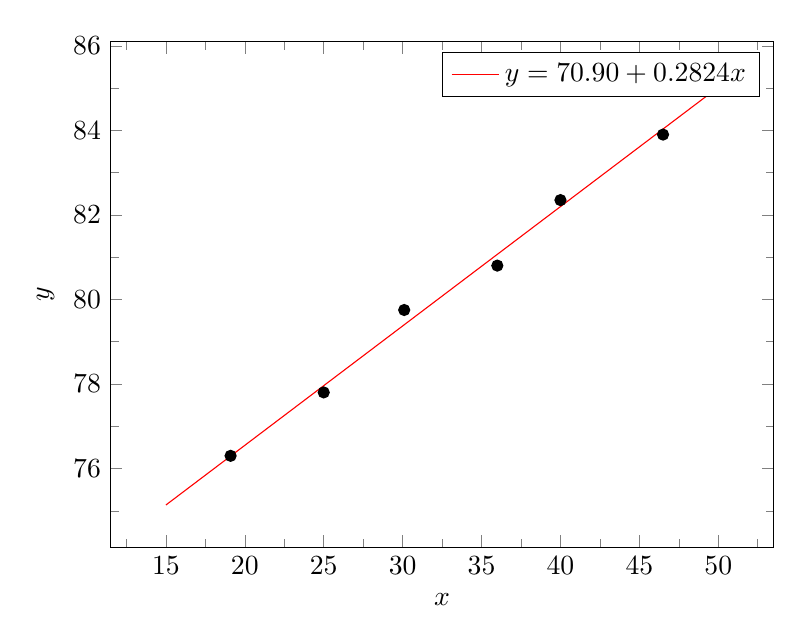
\begin{tikzpicture}
	\begin{axis}[minor tick num=1,width=10cm,height=8cm,xlabel=$ x $,ylabel=$ y $]
	\addplot[domain=15:50,samples=100, color=red,]{0.2824*x+70.90};
	\addlegendentry{$y=70.90+0.2824x$}
	\addplot[only marks] coordinates {
		(19.1,76.30)
		(25.0,77.80)
		(30.1,79.75)
		(36.0,80.80)
		(40.0,82.35)
		(46.5,83.90)
		(50.0,85.10)
	};
	\end{axis}
	\end{tikzpicture}
	\caption{电阻与温度关系回归图}
\end{figure}
前面我们讲到的,都是采用传统的数据分析方法,这样的方法费时费力,效率不高,我们使用Matlab进行数据处理,利用程序可以重复解决很多复杂的数学问题,我们会在后面讲到。
\section{Matlab程序设计和GUI设计\scite{2}}
Matlab是一个功能极其强大的数据处理软件,传统的数据分析和处理都是人工计算,在面对一些复杂的计算时,会耗费大量的时间和精力,这就使效率低下。利用计算机进行数据处理,可以将一些重复的、复杂的计算快速准确地进行。利用计算机处理数据,除了可以省时省力外,可以将做过一次数据处理的源码保存下来,下一次进行同类型数据处理的时候可以重复利用。Matlab不仅仅可以进行数据处理,它还支持人机交互界面的设计,也就是Matlab的图形用户界面GUI(Graphical User Interface)。这就使得数据处理变的直观,非专业人士也可以轻松地使用别人开发好的GUI数据处理程序来完成一些数据的分析与处理。
\subsection{Matlab基本操作}
\subsubsection{Matlab的数据基础}
在Matlab软件中,用数组和cell数组的形式来存储任何数据,所有的数据处理是基于变量的操作。
\begin{enumerate}
	\item \textbf{数组}
	\begin{enumerate}
		\item 一维数组
		
		\qquad 数组就是数据的有序集合,一维数组可以看成向量,在处理的时候可以对一组有联系的数据以数组的形式赋值给变量。常用创建数组和获取数组数据的形式如下:
		\begin{lstlisting}
 >> a = [1 2 3 4 5];			% 直接输入创建一维数组,元素可以用空格或逗号隔开
    a = 
		1	2	3	4	5
 >> b = 1:2:9;					% 利用start:step:end 形式创建一维数组
	b =
		1	3	5	7	9
 >> a(3)						% 用变量名加下标的形式获取数组元素
 	ans = 
 		3\end{lstlisting}
		\item 二维数组
		
		\qquad 二维数组可以作为矩阵,在一维数组上增加一具维度,常用的创建和获取数组数据方法如下:
		\begin{lstlisting}
 >> a = [1 2 3;4 5 6;7 8 9]		% 直接输入创建二维数组,用“ ; ”换行
    a = 
    	1	2	3
    	4	5	6
    	7	8	9
 >> b = [1 2 3					% 直接输入创建二维数组,手动换行
 		 4 5 6
 		 7 8 9]
	b = 
	 	1	2	3
	 	4	5	6
	 	7	8	9
 >> a(2,2)						% 用变量名加下标来获取元素,二维数组用行数和列数来确定元素
 	ans = 
 		5\end{lstlisting}
	\end{enumerate}
	\item \textbf{cell数组}
	
	\qquad cell数组也是数组,它也可以是一维和二维,它的特殊之处就是它可以存放任何数据,也就是说它的元素可以是字符串,单个数据,甚至是数组。cell数组的使用方法如下:
	\begin{lstlisting}
 >> a = [1 2 3 4 5];				% 创建一维数组
 >> b = [1 2 3;4 5 6;7 8 9];		% 创建二维数组
 >> c = 'hello';					% 创建字符串
 >> d = {a,b,c}						% 赋值给 cell 数组
 	d = 
 		[1x5 double]	[3x3 double]	'Hello'
 >> d(1)							% 获取元素用“ ( ) ”,不能获取内容
 	ans =
 		[1x5 double]
 >> d{1}							% 获取元素内容用“ { } ”
 	ans =
 		1	2	3	4	5\end{lstlisting}
\end{enumerate}
\subsubsection{Matlab常用函数}
Matlab计算功能之所以强大,是因为它拥有很多的工具箱,里面封装了许多用于处理数据的函数,我们掌握如何使用这些函数,就掌握了Matlab的使用。在误差理论与数据处理中,我们常用的Matlab函数如下表:
\begin{figure}[H]
	\centering
	\begin{tabular}{p{3cm}<{\centering}p{8cm}}
		\toprule
		\textbf{函数}&\multicolumn{1}{c}{\textbf{作用}}	\\
		\midrule
		length(a)	&获取一维数组的长度\\
		size(A)	&获取二维数组的行与列\\
		max(A)	&获取数组A的最大值\\
		min(A)	&获取数组A的最小值\\
		mean(A)	&获取数组A的平均值\\
		sqrt(n)	&获取数值n的算术平方根\\
		std(X)	&获取数据X的标准差\\
		inv(A)	&获取矩阵的逆矩阵\\
		floor(x)	&获取小于x的最大整数\\
		ceil(x)	&获取大于x的最小整数\\
		roundn(x,n)	&对x进行四舍五入,数据精度为$ 10^n $\\
		\bottomrule
	\end{tabular}
	\captionsetup{type=table}
	\caption{Matlab常用误差处理函数}
\end{figure}
\subsubsection{Matlab绘制图像}
无论是处理数据和误差分析,还是进行别的数学计算处理的时候,绘制函数图形能更直接地了解数据的特性,也可以更直接地描述出计算的结果。在Matlab中,绘制函数图形的功能也是很强大的。在Matlab中常用绘图方法:
\begin{lstlisting}
 >> x = 0:0.01:2*pi;					% 产生一组数据 x
 >> y = sin(x);							% 用 sin 函数产生 y
 >> plot(x,y,'-b')						% 绘制函数图像,‘ - ’设置线条类型,‘ b ’设置颜色
 >> grid on								% 设置显示网格
 >> title('the function of sin')		% 设置图像标题
 >> xlabel('x')							% 设置 x 坐标名称
 >> ylabel('y')							% 设置 y 坐标名称\end{lstlisting}
 绘制的结果如下图:
\begin{figure}[H]
	\centering
	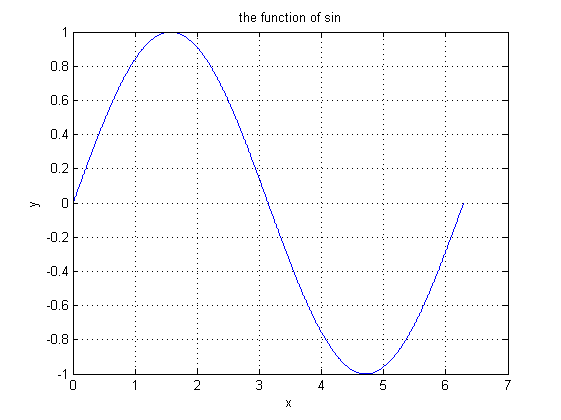
\includegraphics[scale=0.6]{sin_x}
	\caption{$ sin(x) $的函数图像}
\end{figure}
\subsubsection{Matlab的m文件}
Matlab编写的代码是以.m结尾的文件格式,m文件分为两种,m脚本文件和m函数文件。将执行的命令集写在m脚本文件中,直接在命令窗口输入文件名即可运行脚本文件,为了使文件不与Matlab自带的命令冲突,不要把文件命名与Matlab自带命令名称一致。编写脚本如下:
\begin{lstlisting}
   x = 0:0.01:2*pi;
   y = sin(x);
   plot(x,y,'-b')
   grid on
   title('the function of sin')
   xlabel('x')
   ylabel('y')\end{lstlisting}
将上面代码保存为plotsin.m文件,在命令窗口输入plotsin也可以绘制出图7函数图像。

还有一种是m函数文件,它在文件内部定义一个函数,由外界调取该函数进行计算,不可以单独运行,定义的函数名称要与文件名称一致,且不能与Matlab自带函数名称冲突。编写代码如下:
\begin{lstlisting}
 function sum = adds(x, y)
 sum = x + y;\end{lstlisting}
将上面代码保存为adds.m文件,在命令窗口输入adds(3,4),执行结果如下:
\begin{lstlisting}
 >> adds(3,4)
 	ans =
		 7\end{lstlisting}
\subsection{Matlab GUI设计}
在Matlab中,GUI设计有两种方法,一种是用代码实现界面的编程,还有一种是使用GUIDE图形界面设计,前者虽然编写代码量较大,界面的绘制都用代码实现,但在重复设计上有优势,比如大部分控件拥有相同的属性,我们可以用循环来设置。后者虽然操作简单,界面绘制布局可视化,但在控件多的情况下,重复设置属性就比较麻烦了。在本毕业设计中,采用的前种设计方法。在Matlab中图形界面的层次结构\footnote{引用参考文献[2]第9章Matlab GUI的组成与结构第183页}如下图:
\begin{figure}[H]
	\centering
	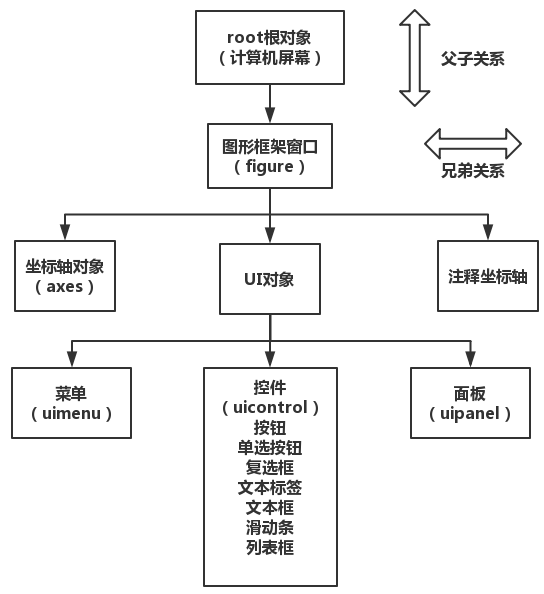
\includegraphics[scale=0.5]{MatlabGUI}
	\caption{GUI对象层次结构图}
\end{figure}
\subsubsection{Matlab中设计GUI的函数}

\subsubsection{Matlab中GUI控件的设计}
\subsubsection{Matlab中回调函数的编写}
\subsubsection{Matlab文件的读取与保存}
\part*{结论}
\addcontentsline{toc}{part}{结论}
本设计基于Matlab GUI的误差理论与数据处理系统设计。设计包括测量数据基本处理、误差的合成、测量不确定度、最小二乘法处理、回归分析五个部分。通过GUI界面的设计和数据处理的算法设计,通过实例验证,整个系统不仅实现了误差处理,还实现了数据的导入、显示和保存。本设计采用M文件编写界面,提高了界面设计的效率,但是在误差处理的算法方面还需更深入。

\part*{致谢}
\addcontentsline{toc}{part}{致谢}
本论文是在我的指导老师密切关心和悉心指导下完成的。老师在课题开题期间和论文写作的过程中给予了我许多指导,导师总是以认真负责、一丝不苟的工作态度阅读并修改文章中不足的地方,她优良的作风和严谨治学的态度深深影响着我,至此,向恩师致以最真挚的感谢和最崇高的敬意!同时还要感谢我的室友,在做毕业设计的过程中,他们给予了我很大的帮助和鼓励。在大学四年里,正是有了他们的无私帮助,才让我不断的成长。最后还要感谢我的母校,感谢您对我的培养。
\part*{致谢}
\addcontentsline{toc}{part}{致谢}
\begin{thebibliography}{0}
\addcontentsline{toc}{part}{参考文献}
\zihao{5}
	\bibitem{1} 蒋萍,赵建玉,魏军.误差理论与数理统计[M].北京:国防工业出版社,2014:1-214.
	\bibitem{2} 陈垚光,毛涛涛,王正林,王玲.精通MATLAB-GUI设计(第2版)[M].北京:电子工业出版社,2011:182-262.
\end{thebibliography}
\part*{附录}
\addcontentsline{toc}{part}{附录}
\begin{center}
	\textbf{附录A 狄克逊检验统计量和临界值}
\end{center}

\centering
\begin{tabular}{|p{4cm}<{\centering}|p{2cm}<{\centering}|p{2cm}<{\centering}|p{2cm}<{\centering}|p{2cm}<{\centering}|}
	\hline
	统计量&$ n $& 0.10&\tabincell{c}{$\alpha$\\0.05 }& 0.01 \\	\hline
	\multirow{5}*{\tabincell{l}{$ r_{10}=\frac{x_{(n)}-x_{(n-1)}}{x_{(n)}-x_{(1)}}$\\$r'_{10}=\frac{x_{(1)}-x_{(2)}}{x_{(1)}-x_{(n)}} $}}														&3	&0.886	&0.941	&0.988	\\	\cline{2-5}
	&4	&0.679	&0.765	&0.889	\\	\cline{2-5}
	&5	&0.557	&0.642	&0.780	\\	\cline{2-5}
	&6	&0.482	&0.560	&0.698	\\	\cline{2-5}
	&7	&0.434	&0.507	&0.637	\\	\hline
	\multirow{3}*{\tabincell{l}{$ r_{11}=\frac{x_{(n)}-x_{(n-1)}}{x_{(n)}-x_{(2)}} $\\$ r'_{11}=\frac{x_{(1)}-x_{(2)}}{x_{(1)}-x_{(n-1)}} $}}														&8	&0.479	&0.554	&0.683	\\	\cline{2-5}
	&9	&0.441	&0.512	&0.635	\\	\cline{2-5}
	&10	&0.409	&0.447	&0.597	\\	\hline
	\multirow{3}*{\tabincell{l}{$ r_{21}=\frac{x_{(n)}-x_{(n-2)}}{x_{(n)}-x_{(2)}} $\\$ r'_{21}=\frac{x_{(1)}-x_{(3)}}{x_{(1)}-x_{(n-1)}} $}}														&11	&0.517	&0.576	&0.670	\\	\cline{2-5}
	&12	&0.490	&0.546	&0.642	\\	\cline{2-5}
	&13	&0.467	&0.521	&0.615	\\	\hline
	\multirow{17}*{\tabincell{l}{$ r_{22}=\frac{x_{(n)}-x_{(n-2)}}{x_{(n)}-x_{(3)}} $\\$ r'_{22}=\frac{x_{(1)}-x_{(3)}}{x_{(1)}-x_{(n-2)}} $}}														&14	&0.492	&0.548	&0.641	\\	\cline{2-5}
	&15	&0.472	&0.525	&0.616	\\	\cline{2-5}
	&16	&0.454	&0.507	&0.595	\\	\cline{2-5}
	&17	&0.438	&0.490	&0.577	\\	\cline{2-5}
	&18	&0.424	&0.475	&0.561	\\	\cline{2-5}
	&19	&0.412	&0.462	&0.547	\\	\cline{2-5}
	&20	&0.401	&0.450	&0.535	\\	\cline{2-5}
	&21	&0.391	&0.440	&0.524	\\	\cline{2-5}
	&22	&0.382	&0.430	&0.514	\\	\cline{2-5}
	&23	&0.374	&0.421	&0.505	\\	\cline{2-5}
	&24	&0.367	&0.413	&0.497	\\	\cline{2-5}
	&25	&0.360	&0.406	&0.489	\\	\cline{2-5}
	&26	&0.354	&0.399	&0.486	\\	\cline{2-5}
	&27	&0.348	&0.393	&0.475	\\	\cline{2-5}
	&28	&0.342	&0.387	&0.469	\\	\cline{2-5}
	&29	&0.337	&0.381	&0.463	\\	\cline{2-5}
	&30	&0.332	&0.378	&0.457	\\	\hline
\end{tabular}
\newpage
\begin{center}
	\textbf{附录B GUI设计函数常用属性\footnote{参考文献[2]第9章Matlab GUI的组成与结构第196页}}
\end{center}
\begin{tabular}{|p{3cm}|p{5cm}|p{5cm}|}
	\hline
	\multicolumn{1}{|c|}{\textbf{对象属性}}	&\multicolumn{1}{c}{\textbf{意义}}	&\multicolumn{1}{|c|}{\textbf{取值及含义}}\\	\hline
	BackgroundColor	&uicontrol背景色。3元素的RGB向量或Matlab预先定义的颜色名称	&默认的背景色是浅灰色		\\	\hline
	Callback		&Matlab回调串,当uicontrol激活时,回调串传给函数eval	   &初始值为空矩阵			\\	\hline
	Max				&属性Value的最大许可值									 &默认值为1				\\	\hline
	Min				&属性Value的最小许可值									 &默认值为0				\\	\hline
	Position		&位置向量[left bottom width height]					   	&					    \\	\hline
	String			&文本字符串,uicontrol显示的文本						    &					 \\	\hline
	Style			&定义uicontrol的类型					&text,edit,pushbutton...				\\	\hline
	Units			&设置属性值的单位										&pixels:屏幕像素		\\	\hline
	Value			&uicontrol的当前值										&文本对象和按钮不设置该属性	\\	\hline
	UserData		&用户指定的数据。可以是矩阵、字符串等						&						\\	\hline
	Tag				&文本串												&						\\	\hline
	CreateFcn		&对象创建时执行的回调函数								&						\\	\hline
	DeleteFcn		&对象删除时执行的回调函数								&						\\	\hline
	CloseRequestFcn		&窗口关闭时执行的回调函数							&						\\	\hline
	ButtonDownFcn		&对象鼠标单击时执行的回调函数						  &						\\	\hline
\end{tabular}
\newpage
\begin{center}
	\textbf{附录C 界面设计代码}
\end{center}
\begin{enumerate}
	\item 设置界面图标:icon.m
	\begin{lstlisting}
 % 更改界面左上角图标
 newIcon = javax.swing.ImageIcon('./image/logo.png');
 figFrame = get(gcf,'JavaFrame');
 figFrame.setFigureIcon(newIcon);\end{lstlisting}
	\item 界面返回:page\_exit.m
	\begin{lstlisting}
 %% 返回上一级菜单
 close(gcf);
 clear all
 clc\end{lstlisting}
 	\item 主界面:index.m
	\begin{lstlisting}
 function index
 clear
 clc
 
 % 添加子文件夹路径
 addpath(genpath(pwd));
 
 %% 创建主界面
 s = get(0,'ScreenSize');% 获取计算机屏幕分辨率
 x = s(3)*0.15;
 y = s(4)*0.26;
 hf = figure('Name','基于GUI的误差理论与数据处理系统',...
     'NumberTitle','off',...
     'Units','pixels',...
     'Position',[x,y,600,450],...
     'MenuBar','none',...
     'Color','White',...
     'CloseRequestFcn',@hexit,...
     'Resize','off');
 
 % 更改界面左上角图标
 icon;
 
 % 学校名称
 axes('Units','pixels',...
     'Position',[0,350,430,100],...
     'CreateFcn',@school_logo);
 
 % 校训
 uicontrol(hf,...
     'Units','pixels',...
     'Position',[300,320,230,25],...
     'Style','text',...
     'String','崇德博智,扶危定倾',...
     'FontName','楷体',...
     'FontSize',18,...
     'FontWeight','bold',...
     'ForegroundColor',[7,51,123]/255,...
     'BackgroundColor','White');
 
 % 学校标志性建筑
 axes('Units','pixels',...
     'Position',[0,80,600,233],...
     'CreateFcn','imshow(''image/school.jpg'')');
 
 %% 一级菜单按钮
 uicontrol(hf,...
     'Units','pixels',...
     'Position',[160,35,280,25],...
     'Style','text',...
     'String','《误差理论与数据处理》',...
     'FontName','楷体',...
     'FontSize',18,...
     'FontWeight','bold',...
     'ForegroundColor',[7,51,123]/255,...
     'BackgroundColor','White',...
     'enable','inactive',...
     'ButtonDownFcn','subpage');
 uicontrol(hf,...
     'Units','pixels',...
     'Position',[160,5,280,25],...
     'Style','text',...
     'String','Error Theory and Data Processing',...
     'FontSize',12,...
     'FontWeight','bold',...
     'ForegroundColor',[7,51,123]/255,...
     'BackgroundColor','White',...
     'enable','inactive',...
     'ButtonDownFcn','subpage');
 
 % 显示学校名称PNG图片函数
 function school_logo(a,b)
 [I,c,alpha] = imread('image/school_logo.png');
 h = imshow(I);
 set(h,'AlphaData',alpha);
 
 %% 主界面退出对话框
 function hexit(a,b)
 he = questdlg('你确定退出吗?','退出程序','是','否','否');
 if strcmp(he,'是')
     close;
     clear;
     clc;
 end;\end{lstlisting}
 \newpage
	\item 二级子界面:subpage.m
	\begin{lstlisting}
 function subpage
 clear
 clc
 
 %% 创建主界面
 s = get(0,'ScreenSize');% 获取计算机屏幕分辨率
 x = s(3)*0.15;
 y = s(4)*0.26;
 hf = figure('Name','基于GUI的误差理论与数据处理系统',...
     'NumberTitle','off',...
     'Units','pixels',...
     'Position',[x,y,710,450],...
     'MenuBar','none',...
     'Color','White',...
     'Resize','off');
 
 % 更改界面左上角图标
 icon;
 
 %创建文字项
 t = 1:6;
 menu_string = {'测量数据基本处理','误差的合成','测量不确定度','最小二乘法处理',' 回归分析','返回'};
 menu_position = [0,240,230,25
                  240,240,230,25
                  480,240,230,25
                  0,10,230,25
                  240,10,230,25
                  480,10,230,25];
 %设置文字项属性
 for i = 1:length(t)
     t(i) = uicontrol(hf,...
         'Style','text',...
         'String',menu_string(i),...
         'FontName','微软雅黑',...
         'FontSize',14,...
         'FontWeight','bold',...
         'enable','inactive',...
         'Units','pixels',...
         'Position',menu_position(i,:),...
         'ButtonDownFcn',strcat('subsubpage',num2str(i)));
 end
 
 %创建图片项
 p1 = axes('CreateFcn','bar([2,1,3,5,3]);');
 p2 = axes('CreateFcn','imshow(''image/photo_2.jpg'');');
 p3 = axes('CreateFcn','imshow(''image/photo_3.jpg'');');
 p4 = axes('CreateFcn',@hplot);
 p5 = axes('CreateFcn','imshow(''image/photo_1.jpg'');');
 p = [p1,p2,p3,p4,p5];
 axes_position = [50,290,150,150
                  290,290,150,150
                  530,290,150,150
                  50,60,150,150
                  290,60,150,150];
 
 for i = 1:length(p)
     set(p(i),...
         'Units','pixels',...
         'Position',axes_position(i,:));
 end
 
 % 图片项显示绘图
 function hplot(a,b)
 x = 0:0.1:1;
 y = [-0.447,1.978,3.28,6.16,7.08,7.34,7.66,9.56,9.48,9.3,11.2];
 plot(x,y,'k.','markersize',12);
 hold on;
 axis([0 1.3 -2 16]);
 p3 = polyfit(x,y,3);
 t=0:0.1:1.2;
 s3=polyval(p3,t);
 plot(t,s3,'r');\end{lstlisting}
\end{enumerate}
\newpage
\begin{center}
	\textbf{附录D 误差理论与数据处理算法代码}
\end{center}
\begin{enumerate}
	\item 逖克逊准则粗大误差处理:BlodBig.m
	\begin{lstlisting}
 function data1 = BlodBig(data)
 % 临界值 a = 0.05
 r0 = [0 0 0.941 0.765 0.642 0.560 0.507 0.554 0.512 0.447 0.576 0.546 0.521 0.548 0.525 0.507 0.490 0.475 0.462 0.450 0.440 0.430 0.421  0.413 0.406 0.399 0.393 0.387 0.381 0.378];
 
 n = length(data);
 data_ = sort(data);
 if n<3
     msgbox('数据太少','提示','warn');
     data1 = data;
     return
 elseif n>=3 && n<=7
     r = (data_(n)-data_(n-1))/(data_(n)-data_(1));
     r_ = (data_(1)-data_(2))/(data_(1)-data_(n));
 elseif n>=8 && n<=10
     r = (data_(n)-data_(n-1))/(data_(n)-data_(2));
     r_ = (data_(1)-data_(2))/(data_(1)-data_(n-1));
 elseif n>=11 && n<=13
     r = (data_(n)-data_(n-2))/(data_(n)-data_(2));
     r_ = (data_(1)-data_(3))/(data_(1)-data_(n-1));
 else
     r = (data_(n)-data_(n-2))/(data_(n)-data_(3));
     r_ = (data_(1)-data_(3))/(data_(1)-data_(n-2));
 end
 if r>=r0(n)
     data(data==data_(n)) = [];
 elseif r_>=r0(n)
     data(data==data_(1)) = [];
 end
 data1 = data;\end{lstlisting}
	\item 等精度测量数据误差分析:data\_process1.m
	\begin{lstlisting}
 function [data1,v1,a,a1,s,s1,s1_x,x] = data_process1(data,t_a)
 a = mean(data);
 s = std(data);
 data1 = BlodBig(data);
 
 a1 = mean(data1);
 s1 = std(data1);
 n1 = length(data1);
 v1 = 1:n1;
 for i=1:n1
     v1(i) = data1(i)-a1;
 end
 s1_x = s1/sqrt(n1);
 sigama = t_a*s1_x;
 x = roundn([a1 sigama],-3);\end{lstlisting}
	\item 不等精度测量数据误差分析:data\_process2.m
	\begin{lstlisting}
 function [data1,v2,a1,a2,s1,s2,s2_x,p,x_,s_x_,x] = data_process2(data,t_a)
 s = size(data);
 for i = 1:s(1)
     a1(i) = mean(data{i});
     s1(i) = std(data{i});
     data1{i} = BlodBig(data{i});
 end
 
 for i = 1:s(1)
     a2(i) = mean(data1{i});
     s2(i) = std(data1{i});
     s2_x(i) = s2(i)/sqrt(length(data1{i}));
 end
 % 残差
 n2 = size(data1);
 for i=1:n2(2)
     a = [];
     b = data1{i};
     for j=1:length(b)
         a(j) = b(j)-a2(i);
     end
     v2{i} = a;
 end
 % 权
 for i = 1:s(1)
     p(i) = 1/(s2_x(i)*s2_x(i));
 end
 % 加权算术平均值
 [x_,s_x] = jiaquan(p,a2);
 s_x_ = s2_x(1)*s_x;
 
 sigama = t_a*s_x_;
 x = roundn([x_ sigama],-3);
 
 function [x_,s_x_] = jiaquan(p,x_)
 n = length(p);
 s1 = 0;
 s2 = 0;
 for i = 1:n
     s1 = s1+p(i)*x_(i);
     s2 = s2+p(i);
 end
 x_ = s1/s2;
 s_x_ = sqrt(p(1)/s2);\end{lstlisting}
 \newpage
	\item 等精度测量线性参数最小二乘法处理:data\_process3.m
	\begin{lstlisting}
 function [D,EX,V,V_,s,d_ux] = data_process3(A,L)
 B = A';
 C = B*A;
 D = inv(C);
 EX = D*B*L;
 V = L-A*EX;
 V_ = V'*V;
 
 s = size(A);
 n = s(1);
 t = s(2);
 s = sqrt(V'*V./(n-t));
 
 d = 1:t;
 ux = 1:t;
 for i = 1:t
     d(i) = D(i,i);
     ux(i) = s*sqrt(d(i));
 end
 d_ux = [d' ux'];\end{lstlisting}
	\item 不等精度测量线性参数最小二乘法处理:data\_process4.m
	\begin{lstlisting}
 function [C,D,EX] = data_process4(A,L,P)
 C = A'*P*A;
 D = inv(C);
 EX = D*A'*P*L;\end{lstlisting}
\end{enumerate}

%\part*{引言}
\addcontentsline{toc}{part}{引言}
这是$ x^2+y^2=z^2 $引言。\[ \sum_{i=1}^{\infty}x^i \]

%\input{内容}
%\part*{结论}
\addcontentsline{toc}{part}{结论}
本设计基于Matlab GUI的误差理论与数据处理系统设计。设计包括测量数据基本处理、误差的合成、测量不确定度、最小二乘法处理、回归分析五个部分。通过GUI界面的设计和数据处理的算法设计,通过实例验证,整个系统不仅实现了误差处理,还实现了数据的导入、显示和保存。本设计采用M文件编写界面,提高了界面设计的效率,但是在误差处理的算法方面还需更深入。

\part*{致谢}
\addcontentsline{toc}{part}{致谢}
本论文是在我的指导老师密切关心和悉心指导下完成的。老师在课题开题期间和论文写作的过程中给予了我许多指导,导师总是以认真负责、一丝不苟的工作态度阅读并修改文章中不足的地方,她优良的作风和严谨治学的态度深深影响着我,至此,向恩师致以最真挚的感谢和最崇高的敬意!同时还要感谢我的室友,在做毕业设计的过程中,他们给予了我很大的帮助和鼓励。在大学四年里,正是有了他们的无私帮助,才让我不断的成长。最后还要感谢我的母校,感谢您对我的培养。
%\part*{致谢}
\addcontentsline{toc}{part}{致谢}
%\begin{thebibliography}{0}
\addcontentsline{toc}{part}{参考文献}
\zihao{5}
	\bibitem{1} 蒋萍,赵建玉,魏军.误差理论与数理统计[M].北京:国防工业出版社,2014:1-214.
	\bibitem{2} 陈垚光,毛涛涛,王正林,王玲.精通MATLAB-GUI设计(第2版)[M].北京:电子工业出版社,2011:182-262.
\end{thebibliography}
%\part*{附录}
\addcontentsline{toc}{part}{附录}
\begin{center}
	\textbf{附录A 狄克逊检验统计量和临界值}
\end{center}

\centering
\begin{tabular}{|p{4cm}<{\centering}|p{2cm}<{\centering}|p{2cm}<{\centering}|p{2cm}<{\centering}|p{2cm}<{\centering}|}
	\hline
	统计量&$ n $& 0.10&\tabincell{c}{$\alpha$\\0.05 }& 0.01 \\	\hline
	\multirow{5}*{\tabincell{l}{$ r_{10}=\frac{x_{(n)}-x_{(n-1)}}{x_{(n)}-x_{(1)}}$\\$r'_{10}=\frac{x_{(1)}-x_{(2)}}{x_{(1)}-x_{(n)}} $}}														&3	&0.886	&0.941	&0.988	\\	\cline{2-5}
	&4	&0.679	&0.765	&0.889	\\	\cline{2-5}
	&5	&0.557	&0.642	&0.780	\\	\cline{2-5}
	&6	&0.482	&0.560	&0.698	\\	\cline{2-5}
	&7	&0.434	&0.507	&0.637	\\	\hline
	\multirow{3}*{\tabincell{l}{$ r_{11}=\frac{x_{(n)}-x_{(n-1)}}{x_{(n)}-x_{(2)}} $\\$ r'_{11}=\frac{x_{(1)}-x_{(2)}}{x_{(1)}-x_{(n-1)}} $}}														&8	&0.479	&0.554	&0.683	\\	\cline{2-5}
	&9	&0.441	&0.512	&0.635	\\	\cline{2-5}
	&10	&0.409	&0.447	&0.597	\\	\hline
	\multirow{3}*{\tabincell{l}{$ r_{21}=\frac{x_{(n)}-x_{(n-2)}}{x_{(n)}-x_{(2)}} $\\$ r'_{21}=\frac{x_{(1)}-x_{(3)}}{x_{(1)}-x_{(n-1)}} $}}														&11	&0.517	&0.576	&0.670	\\	\cline{2-5}
	&12	&0.490	&0.546	&0.642	\\	\cline{2-5}
	&13	&0.467	&0.521	&0.615	\\	\hline
	\multirow{17}*{\tabincell{l}{$ r_{22}=\frac{x_{(n)}-x_{(n-2)}}{x_{(n)}-x_{(3)}} $\\$ r'_{22}=\frac{x_{(1)}-x_{(3)}}{x_{(1)}-x_{(n-2)}} $}}														&14	&0.492	&0.548	&0.641	\\	\cline{2-5}
	&15	&0.472	&0.525	&0.616	\\	\cline{2-5}
	&16	&0.454	&0.507	&0.595	\\	\cline{2-5}
	&17	&0.438	&0.490	&0.577	\\	\cline{2-5}
	&18	&0.424	&0.475	&0.561	\\	\cline{2-5}
	&19	&0.412	&0.462	&0.547	\\	\cline{2-5}
	&20	&0.401	&0.450	&0.535	\\	\cline{2-5}
	&21	&0.391	&0.440	&0.524	\\	\cline{2-5}
	&22	&0.382	&0.430	&0.514	\\	\cline{2-5}
	&23	&0.374	&0.421	&0.505	\\	\cline{2-5}
	&24	&0.367	&0.413	&0.497	\\	\cline{2-5}
	&25	&0.360	&0.406	&0.489	\\	\cline{2-5}
	&26	&0.354	&0.399	&0.486	\\	\cline{2-5}
	&27	&0.348	&0.393	&0.475	\\	\cline{2-5}
	&28	&0.342	&0.387	&0.469	\\	\cline{2-5}
	&29	&0.337	&0.381	&0.463	\\	\cline{2-5}
	&30	&0.332	&0.378	&0.457	\\	\hline
\end{tabular}
\newpage
\begin{center}
	\textbf{附录B GUI设计函数常用属性\footnote{参考文献[2]第9章Matlab GUI的组成与结构第196页}}
\end{center}
\begin{tabular}{|p{3cm}|p{5cm}|p{5cm}|}
	\hline
	\multicolumn{1}{|c|}{\textbf{对象属性}}	&\multicolumn{1}{c}{\textbf{意义}}	&\multicolumn{1}{|c|}{\textbf{取值及含义}}\\	\hline
	BackgroundColor	&uicontrol背景色。3元素的RGB向量或Matlab预先定义的颜色名称	&默认的背景色是浅灰色		\\	\hline
	Callback		&Matlab回调串,当uicontrol激活时,回调串传给函数eval	   &初始值为空矩阵			\\	\hline
	Max				&属性Value的最大许可值									 &默认值为1				\\	\hline
	Min				&属性Value的最小许可值									 &默认值为0				\\	\hline
	Position		&位置向量[left bottom width height]					   	&					    \\	\hline
	String			&文本字符串,uicontrol显示的文本						    &					 \\	\hline
	Style			&定义uicontrol的类型					&text,edit,pushbutton...				\\	\hline
	Units			&设置属性值的单位										&pixels:屏幕像素		\\	\hline
	Value			&uicontrol的当前值										&文本对象和按钮不设置该属性	\\	\hline
	UserData		&用户指定的数据。可以是矩阵、字符串等						&						\\	\hline
	Tag				&文本串												&						\\	\hline
	CreateFcn		&对象创建时执行的回调函数								&						\\	\hline
	DeleteFcn		&对象删除时执行的回调函数								&						\\	\hline
	CloseRequestFcn		&窗口关闭时执行的回调函数							&						\\	\hline
	ButtonDownFcn		&对象鼠标单击时执行的回调函数						  &						\\	\hline
\end{tabular}
\newpage
\begin{center}
	\textbf{附录C 界面设计代码}
\end{center}
\begin{enumerate}
	\item 设置界面图标:icon.m
	\begin{lstlisting}
 % 更改界面左上角图标
 newIcon = javax.swing.ImageIcon('./image/logo.png');
 figFrame = get(gcf,'JavaFrame');
 figFrame.setFigureIcon(newIcon);\end{lstlisting}
	\item 界面返回:page\_exit.m
	\begin{lstlisting}
 %% 返回上一级菜单
 close(gcf);
 clear all
 clc\end{lstlisting}
 	\item 主界面:index.m
	\begin{lstlisting}
 function index
 clear
 clc
 
 % 添加子文件夹路径
 addpath(genpath(pwd));
 
 %% 创建主界面
 s = get(0,'ScreenSize');% 获取计算机屏幕分辨率
 x = s(3)*0.15;
 y = s(4)*0.26;
 hf = figure('Name','基于GUI的误差理论与数据处理系统',...
     'NumberTitle','off',...
     'Units','pixels',...
     'Position',[x,y,600,450],...
     'MenuBar','none',...
     'Color','White',...
     'CloseRequestFcn',@hexit,...
     'Resize','off');
 
 % 更改界面左上角图标
 icon;
 
 % 学校名称
 axes('Units','pixels',...
     'Position',[0,350,430,100],...
     'CreateFcn',@school_logo);
 
 % 校训
 uicontrol(hf,...
     'Units','pixels',...
     'Position',[300,320,230,25],...
     'Style','text',...
     'String','崇德博智,扶危定倾',...
     'FontName','楷体',...
     'FontSize',18,...
     'FontWeight','bold',...
     'ForegroundColor',[7,51,123]/255,...
     'BackgroundColor','White');
 
 % 学校标志性建筑
 axes('Units','pixels',...
     'Position',[0,80,600,233],...
     'CreateFcn','imshow(''image/school.jpg'')');
 
 %% 一级菜单按钮
 uicontrol(hf,...
     'Units','pixels',...
     'Position',[160,35,280,25],...
     'Style','text',...
     'String','《误差理论与数据处理》',...
     'FontName','楷体',...
     'FontSize',18,...
     'FontWeight','bold',...
     'ForegroundColor',[7,51,123]/255,...
     'BackgroundColor','White',...
     'enable','inactive',...
     'ButtonDownFcn','subpage');
 uicontrol(hf,...
     'Units','pixels',...
     'Position',[160,5,280,25],...
     'Style','text',...
     'String','Error Theory and Data Processing',...
     'FontSize',12,...
     'FontWeight','bold',...
     'ForegroundColor',[7,51,123]/255,...
     'BackgroundColor','White',...
     'enable','inactive',...
     'ButtonDownFcn','subpage');
 
 % 显示学校名称PNG图片函数
 function school_logo(a,b)
 [I,c,alpha] = imread('image/school_logo.png');
 h = imshow(I);
 set(h,'AlphaData',alpha);
 
 %% 主界面退出对话框
 function hexit(a,b)
 he = questdlg('你确定退出吗?','退出程序','是','否','否');
 if strcmp(he,'是')
     close;
     clear;
     clc;
 end;\end{lstlisting}
 \newpage
	\item 二级子界面:subpage.m
	\begin{lstlisting}
 function subpage
 clear
 clc
 
 %% 创建主界面
 s = get(0,'ScreenSize');% 获取计算机屏幕分辨率
 x = s(3)*0.15;
 y = s(4)*0.26;
 hf = figure('Name','基于GUI的误差理论与数据处理系统',...
     'NumberTitle','off',...
     'Units','pixels',...
     'Position',[x,y,710,450],...
     'MenuBar','none',...
     'Color','White',...
     'Resize','off');
 
 % 更改界面左上角图标
 icon;
 
 %创建文字项
 t = 1:6;
 menu_string = {'测量数据基本处理','误差的合成','测量不确定度','最小二乘法处理',' 回归分析','返回'};
 menu_position = [0,240,230,25
                  240,240,230,25
                  480,240,230,25
                  0,10,230,25
                  240,10,230,25
                  480,10,230,25];
 %设置文字项属性
 for i = 1:length(t)
     t(i) = uicontrol(hf,...
         'Style','text',...
         'String',menu_string(i),...
         'FontName','微软雅黑',...
         'FontSize',14,...
         'FontWeight','bold',...
         'enable','inactive',...
         'Units','pixels',...
         'Position',menu_position(i,:),...
         'ButtonDownFcn',strcat('subsubpage',num2str(i)));
 end
 
 %创建图片项
 p1 = axes('CreateFcn','bar([2,1,3,5,3]);');
 p2 = axes('CreateFcn','imshow(''image/photo_2.jpg'');');
 p3 = axes('CreateFcn','imshow(''image/photo_3.jpg'');');
 p4 = axes('CreateFcn',@hplot);
 p5 = axes('CreateFcn','imshow(''image/photo_1.jpg'');');
 p = [p1,p2,p3,p4,p5];
 axes_position = [50,290,150,150
                  290,290,150,150
                  530,290,150,150
                  50,60,150,150
                  290,60,150,150];
 
 for i = 1:length(p)
     set(p(i),...
         'Units','pixels',...
         'Position',axes_position(i,:));
 end
 
 % 图片项显示绘图
 function hplot(a,b)
 x = 0:0.1:1;
 y = [-0.447,1.978,3.28,6.16,7.08,7.34,7.66,9.56,9.48,9.3,11.2];
 plot(x,y,'k.','markersize',12);
 hold on;
 axis([0 1.3 -2 16]);
 p3 = polyfit(x,y,3);
 t=0:0.1:1.2;
 s3=polyval(p3,t);
 plot(t,s3,'r');\end{lstlisting}
\end{enumerate}
\newpage
\begin{center}
	\textbf{附录D 误差理论与数据处理算法代码}
\end{center}
\begin{enumerate}
	\item 逖克逊准则粗大误差处理:BlodBig.m
	\begin{lstlisting}
 function data1 = BlodBig(data)
 % 临界值 a = 0.05
 r0 = [0 0 0.941 0.765 0.642 0.560 0.507 0.554 0.512 0.447 0.576 0.546 0.521 0.548 0.525 0.507 0.490 0.475 0.462 0.450 0.440 0.430 0.421  0.413 0.406 0.399 0.393 0.387 0.381 0.378];
 
 n = length(data);
 data_ = sort(data);
 if n<3
     msgbox('数据太少','提示','warn');
     data1 = data;
     return
 elseif n>=3 && n<=7
     r = (data_(n)-data_(n-1))/(data_(n)-data_(1));
     r_ = (data_(1)-data_(2))/(data_(1)-data_(n));
 elseif n>=8 && n<=10
     r = (data_(n)-data_(n-1))/(data_(n)-data_(2));
     r_ = (data_(1)-data_(2))/(data_(1)-data_(n-1));
 elseif n>=11 && n<=13
     r = (data_(n)-data_(n-2))/(data_(n)-data_(2));
     r_ = (data_(1)-data_(3))/(data_(1)-data_(n-1));
 else
     r = (data_(n)-data_(n-2))/(data_(n)-data_(3));
     r_ = (data_(1)-data_(3))/(data_(1)-data_(n-2));
 end
 if r>=r0(n)
     data(data==data_(n)) = [];
 elseif r_>=r0(n)
     data(data==data_(1)) = [];
 end
 data1 = data;\end{lstlisting}
	\item 等精度测量数据误差分析:data\_process1.m
	\begin{lstlisting}
 function [data1,v1,a,a1,s,s1,s1_x,x] = data_process1(data,t_a)
 a = mean(data);
 s = std(data);
 data1 = BlodBig(data);
 
 a1 = mean(data1);
 s1 = std(data1);
 n1 = length(data1);
 v1 = 1:n1;
 for i=1:n1
     v1(i) = data1(i)-a1;
 end
 s1_x = s1/sqrt(n1);
 sigama = t_a*s1_x;
 x = roundn([a1 sigama],-3);\end{lstlisting}
	\item 不等精度测量数据误差分析:data\_process2.m
	\begin{lstlisting}
 function [data1,v2,a1,a2,s1,s2,s2_x,p,x_,s_x_,x] = data_process2(data,t_a)
 s = size(data);
 for i = 1:s(1)
     a1(i) = mean(data{i});
     s1(i) = std(data{i});
     data1{i} = BlodBig(data{i});
 end
 
 for i = 1:s(1)
     a2(i) = mean(data1{i});
     s2(i) = std(data1{i});
     s2_x(i) = s2(i)/sqrt(length(data1{i}));
 end
 % 残差
 n2 = size(data1);
 for i=1:n2(2)
     a = [];
     b = data1{i};
     for j=1:length(b)
         a(j) = b(j)-a2(i);
     end
     v2{i} = a;
 end
 % 权
 for i = 1:s(1)
     p(i) = 1/(s2_x(i)*s2_x(i));
 end
 % 加权算术平均值
 [x_,s_x] = jiaquan(p,a2);
 s_x_ = s2_x(1)*s_x;
 
 sigama = t_a*s_x_;
 x = roundn([x_ sigama],-3);
 
 function [x_,s_x_] = jiaquan(p,x_)
 n = length(p);
 s1 = 0;
 s2 = 0;
 for i = 1:n
     s1 = s1+p(i)*x_(i);
     s2 = s2+p(i);
 end
 x_ = s1/s2;
 s_x_ = sqrt(p(1)/s2);\end{lstlisting}
 \newpage
	\item 等精度测量线性参数最小二乘法处理:data\_process3.m
	\begin{lstlisting}
 function [D,EX,V,V_,s,d_ux] = data_process3(A,L)
 B = A';
 C = B*A;
 D = inv(C);
 EX = D*B*L;
 V = L-A*EX;
 V_ = V'*V;
 
 s = size(A);
 n = s(1);
 t = s(2);
 s = sqrt(V'*V./(n-t));
 
 d = 1:t;
 ux = 1:t;
 for i = 1:t
     d(i) = D(i,i);
     ux(i) = s*sqrt(d(i));
 end
 d_ux = [d' ux'];\end{lstlisting}
	\item 不等精度测量线性参数最小二乘法处理:data\_process4.m
	\begin{lstlisting}
 function [C,D,EX] = data_process4(A,L,P)
 C = A'*P*A;
 D = inv(C);
 EX = D*A'*P*L;\end{lstlisting}
\end{enumerate}

%% 绘图
%\begin{center}
%	\begin{tikzpicture}
%	\begin{axis}[axis lines = left,xlabel = $x$,ylabel = {$f(x)$},]
%	%Below the red parabola is defined
%	\addplot[domain=-10:10,samples=100, color=red,]{x^2 - 2*x - 1};
%	\addlegendentry{$x^2 - 2x - 1$}
%	%Here the blue parabloa is defined
%	\addplot[domain=-10:10, samples=100, color=blue,]{x^2 + 2*x + 1};
%	\addlegendentry{$x^2 + 2x + 1$}
%	\end{axis}
%	\end{tikzpicture}
%\end{center}
%
%\newpage
%
%\begin{pspicture}(1.5,1em)
%\psline(0,0)(1,1em)(1.5,0)
%\end{pspicture}
%
%\newpage
%

\end{document}